% The Local Path Not Taken -- working draft (IEEEtran conference format).
% Compile: pdflatex paper.tex  (figures live in paper/figures/; run paper/make_figures.py first).
% Swap \documentclass to acmart for ACM venues (IMC/PAM) if needed.
\documentclass[conference]{IEEEtran}
\IEEEoverridecommandlockouts
\usepackage{cite}
\usepackage{graphicx}
\usepackage{booktabs}
\usepackage{amsmath,amssymb}
\usepackage[hidelinks]{hyperref}
\usepackage{url}
\graphicspath{{figures/}}

\begin{document}

\title{The Local Path Not Taken: Measuring Domestic-Traffic\\
Hairpinning and PKIX Underuse in Pakistan}

\author{\IEEEauthorblockN{Rayan Atif}
\IEEEauthorblockA{Lahore University of Management Sciences (LUMS)\\
Supervised by Dr.\ Saqib Ilyas~~$\cdot$~~Funded by the APNIC Foundation\\
\texttt{rayan.atif2@gmail.com}}}

\maketitle

\begin{abstract}
Pakistan operates an Internet Exchange (PKIX) at four locations with dozens of connected
members, yet its route server appears in \emph{zero} of the BGP paths we observe to Pakistani
destinations. We ask, with active measurement from inside the country, whether this underuse
actually costs Pakistani users---and find that it does, twice over. Using RIPE Atlas probes in
14 Pakistani networks, we (i)~census where the top Pakistani websites are hosted, (ii)~introduce
a \emph{geo-IP-proof, RTT-physics} detector for path \emph{tromboning} (domestic traffic that
leaves the country and returns) and run a \emph{complete block-level census of every small
Pakistani ISP}, and (iii)~measure the latency and resilience cost of the resulting routing.
We find that ${\sim}40\%$ of the top sites are not on a Pakistani server; that $11\%$ of
small-ISP address space is reachable only by hairpinning abroad---a rate driven far more by
\emph{which ISP you measure from} than by the destination---and that the hairpin path is a
\emph{choice}: the same address is reached locally from one transit and abroad from another.
The penalty is a stable, structural $3$--$9\times$ latency increase (no diurnal cycle), and
during a real submarine-cable fault (SMW5, July~2026) international paths degraded---chiefly as
a $+31\%$ jitter increase---while domestically-routed traffic was untouched. The through-line
is one sentence: \emph{the local path exists but is not taken}, and PKIX is the instrument that
would take it.
\end{abstract}

\section{Introduction}
Only two operators---\textbf{PTCL} (AS17557) and \textbf{Transworld} (AS38193)---are licensed
to sell international transit in Pakistan; every other ISP buys upstream from them. A
consequence is that two domestic ISPs with no direct peering typically reach each other
\emph{through} an international operator, and domestic traffic frequently \emph{hairpins} abroad
and back even when both endpoints sit in the same city. An Internet Exchange is the standard
remedy, and Pakistan has one: PKIX runs at Islamabad, Karachi, Lahore, and a PTCL datacenter,
with $21/14/18$ members listed per site (PTA, 2026). Its own figures show inter-ISP latency
collapsing from $100$--$144$\,ms internationally to $1$--$31$\,ms through the exchange. And yet
the PKIX route server (AS140307) is absent from every BGP path we see to Pakistani
networks---the exchange is built but, for most members, not \emph{used}.

This paper measures the consequences of that underuse from the data plane. Our contributions:
\begin{enumerate}
  \item A \textbf{hosting census} of the top Pakistani websites (where content physically lives).
  \item A \textbf{geo-IP-proof RTT-physics detector} for tromboning, and a \textbf{complete
        census} of hairpinning across the entire small-ISP population---who hairpins whom,
        through which international operator, to where.
  \item The \textbf{cost}: the latency penalty of offshore/hairpin routing (stable and
        structural), evidence that a \emph{domestic path exists but is not chosen}, and the
        \textbf{resilience} loss during a live submarine-cable fault.
\end{enumerate}
Framed in the language of prior IXP work, we quantify how often Pakistani ISPs make the
\emph{wrong routing choice}---sending domestic traffic abroad when a local path is available.

\section{Related Work}
Di Bartolomeo et al.~\cite{dibartolomeo2015} compare IXP vs upstream paths for Italian ISPs
using RIPE Atlas and controlled BGP announcements, finding IXP paths give better, more stable
latency and preserve traffic locality; our study mirrors their vantage (national probes $\to$
national targets) and their locality-as-sovereignty framing, but replaces hand-picked targets
with a \emph{complete prefix census} and a detector that does not trust geo-IP. Gupta et
al.~\cite{gupta2014} show African ISPs that do not peer locally send domestic traffic
\emph{detouring through Europe}---precisely the tromboning we measure in Pakistan. Prefix-based
target selection follows the selective-scanning approach~\cite{klick2016}: all IPs in an
announced prefix share one BGP route, so a few IPs per block is routing-complete. Large-IXP
studies~\cite{ager2012,chatzis2013} motivate why peering matters. We build on RIPE
Atlas~\cite{ripeatlas}, RIPEstat~\cite{ripestat}, and Team Cymru with an RDAP fallback for ASN
and registry resolution.

\section{Data and Vantages}
We measure from \textbf{14 connected RIPE Atlas probes} inside Pakistani networks, spanning both
international operators and their downstreams: PTCL ($\times3$, incl.\ a LUMS anchor), Transworld
and its retail arm TES, Cybernet ($\times3$, two cities), Nayatel ($\times2$), Nova/TPCPL
(transits Transworld), Fasttel, Orbit, and Z-Com. Two probes (a PTCL anchor and a Transworld
backbone probe) are \emph{ICMP-filtered}---their path is invisible, so we use ping for their
RTT---and one PTCL probe runs in a container that exposes only two hops (valid RTT, opaque
path). We flag these throughout. Targets vary per experiment: the top-100 Pakistani websites
(hosting), 8 spread IPs in every announced /24 of every small ISP (tromboning census), a fixed
local/offshore panel (longitudinal), and a balanced CDN/Abroad/PK sample during the outage.

\textbf{Measurement framework and its evolution.} Our mature framework---used from the
tromboning experiments onward---creates measurements with the official RIPE Atlas libraries
(cousteau/sagan), uses \textbf{TCP/80 Paris traceroute} for the path (ICMP is heavily filtered
in Pakistani networks and undercounts responses---in our first ISP only $12/52$ targets replied
to ICMP) with a \textbf{ping} companion for end-to-end RTT (the \textbf{min-of-$N$} for a
noise-free level; jitter as the round-to-round standard deviation), and classifies routing
with the RTT-physics detector of Sec.~\ref{sec:detect}. Our four key indicators follow prior IXP work~\cite{dibartolomeo2015}:
\textbf{RTT, hop count, jitter, and packet loss}. We are candid that the early experiments
(hosting and the longitudinal pilot) \emph{predate} this framework: they hand-rolled the REST
API with ICMP Paris traceroute, a single-packet RTT, and geo-IP classification. Where those
runs feed a quantitative comparison we \textbf{re-derive RTT as min-of-$N$ and re-classify
routing with the RTT-physics detector from the archived raw results}; differences that cannot
be recomputed (an ICMP path is not a TCP path; a probe absent from a past run cannot be added)
are flagged in place. A single \emph{uniform} four-indicator, per-ISP comparison across all
vantages is therefore reserved for the longitudinal panel (Sec.~\ref{sec:conclusion}), the only
run that carries all four indicators from every probe under one method.

\section{Method: an RTT-Physics Tromboning Detector}
\label{sec:detect}
\textbf{The problem with geo-IP.} Registration country lies at exactly the hops that matter. A
``Canadian'' Shaw address (AS6327) and a ``US'' Cogent address (AS174) both sit
\emph{physically in Pakistan} at ${\sim}2$\,ms---Cogent even runs a domestic PoP used as an
interconnect fabric---so a country-of-ASN test flags in-country hops as foreign. Conversely a
genuinely foreign exit hop often does not resolve in BGP at all (Transworld's international
egress at Equinix Singapore is unannounced; only RDAP/hostname reveals it). A detector that
trusts geo-IP is wrong in both directions.

\textbf{The detector.} We decide tromboning by \textbf{RTT physics}, not hop country. A trace
\emph{left Pakistan} if any responding hop is foreign with RTT $\geq 40$\,ms, \emph{or} there is
a $\geq 60$\,ms jump between consecutive hops, \emph{or} any hop RTT $\geq 70$\,ms; a path whose
maximum RTT stays $< 45$\,ms is \emph{local}. We ignore RTTs $> 500$\,ms (queuing /
ICMP-error-generation artefacts, endemic on filtered probes---there we use ping min-of-$N$) and
exclude the Shaw/Cogent artefact ASNs. The $40$\,ms floor is the physical round-trip to the
nearest foreign exchange; the jump backstop catches invisible foreign hops.

\textbf{Validation.} On our first target (Worldcall) a na\"ive geo-IP test flagged $53/53$ paths
as foreign; the RTT-physics detector reduces this to a clean $16/52$, matching manual inspection
of the hop-by-hop RTTs. We report this agreement before quoting any rate.

\section{Where Pakistani Content Lives}
\label{sec:host}
\emph{Provenance: a DNS + ASN hosting snapshot from a legacy experiment; hosting location is a
name/registration property (geo-IP), distinct from the RTT-proven routing analysis of later
sections. The legacy traceroutes are single-packet ICMP, so we do not retro-fit the RTT-physics
detector onto them; routing to these targets is re-verified under the uniform panel
(Sec.~\ref{sec:conclusion}).}

Combining our two hosting censuses (91 sites; top-100), across \textbf{172 sites} we find
\textbf{$60\%$ hosted in Pakistan, $31\%$ on an anycast CDN} (almost all Cloudflare)
\textbf{and $8\%$ on a real server abroad} (Fig.~\ref{fig:hosting}). The split is strongly
\emph{sector-driven}: government and education stay in-country, while news, banking, and
e-commerce have largely left---Pakistani banks host in the US, Singapore, and Dubai; several
news sites on Hetzner in Finland. Read the CDN slice with care: a low traceroute RTT proves the
\emph{network edge} is local, not that the \emph{content} is---\texttt{shaukatkhanum.org.pk}
traces to a Cloudflare node at ${\sim}4$\,ms yet serves from Singapore (\texttt{colo=SIN}). So
the honest reading is that \textbf{${\sim}40\%$ of top sites are not on a Pakistani server}, and
an unknown fraction of the ``local'' CDN slice is served abroad.

Two supporting results. Per-ISP DNS resolution changes little---only 8 of 103 sites resolve to
different IPs per ISP---so a central lookup is representative for ${\sim}92\%$ of sites and the
census stands. And most large global content (Google, Meta, Apple) is reached at
\emph{regional} latency (${\sim}20$--$50$\,ms), not from inside Pakistan; only Cloudflare and X
were served locally, and only on Nayatel---an ISP-specific peering advantage we return to below.

\begin{figure}[t]
  \centering
  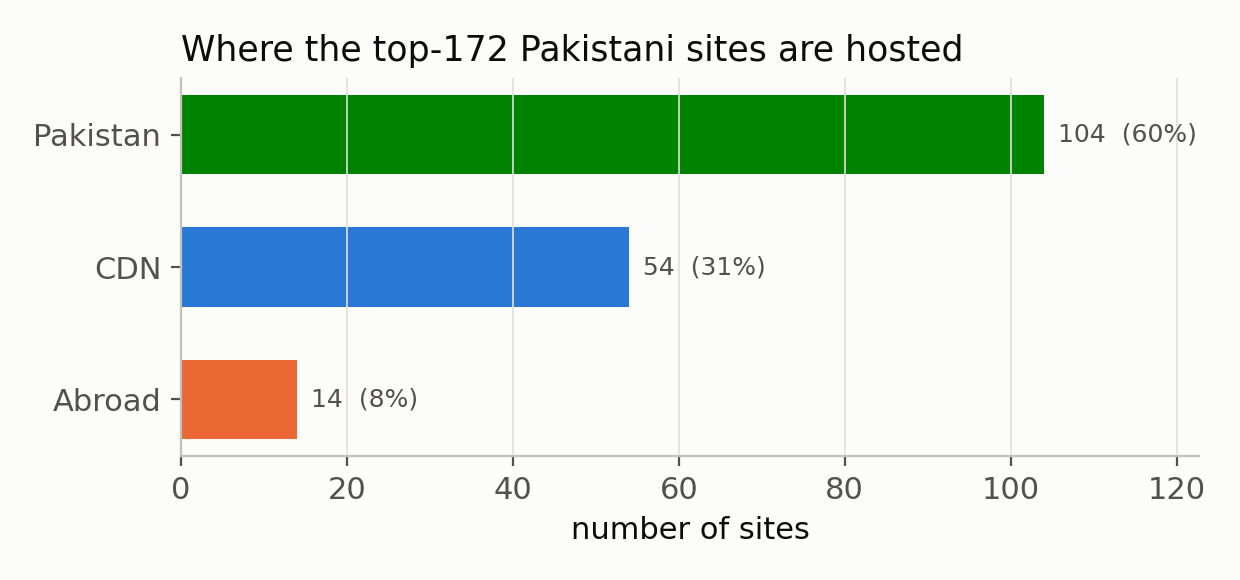
\includegraphics[width=\columnwidth]{fig_hosting_split.png}
  \caption{Where the top-172 Pakistani sites are hosted. CDN counts the network edge, which is
  often local even when the content is served abroad; ${\sim}40\%$ are not on a Pakistani server.}
  \label{fig:hosting}
\end{figure}

\section{Tromboning at Scale}
\label{sec:tromb}
\textbf{Proof on one ISP.} From a Pakistani vantage to \textbf{Worldcall} (AS38710),
\textbf{16 of 52 announced /24s ($31\%$) trombone to Equinix Singapore} via Transworld and
back; the rest stay local via the in-country Cogent PoP. The decisive result: the \emph{same}
Worldcall address \texttt{115.186.61.254} is \textbf{local (${\sim}46$\,ms) from PTCL}---whose
path never touches Transworld---but \textbf{trombones (${\sim}134$\,ms) from Transworld}. A
domestic route exists; Transworld chooses the hairpin. This is the whole thesis in one
measurement.

\textbf{The national census.} Scaling to \emph{every} announced /24 of \emph{every} small (FLL)
Pakistani ISP---$747$ blocks $\times\,8$ spread IPs $\times\,7$ route-visible probes
$=\mathbf{18{,}260}$ \textbf{traces}---we find \textbf{${\sim}11\%$ hairpin abroad and
${\sim}85\%$ stay local} ($807$ inconclusive). Three findings stand out:
\begin{itemize}
  \item \textbf{The source ISP dominates the outcome} (Fig.~\ref{fig:source}). Trombone rate
        depends far more on \emph{where you measure from} than on the destination:
        \textbf{Cybernet-Haripur $46\%$} and \textbf{PTCL-Karachi $38\%$} hairpin most small
        ISPs, while every other vantage routes mostly local ($4$--$10\%$), and
        \textbf{Nayatel is cleanest at $4\%$}. The same Cybernet ISP hairpins $46\%$ from
        Haripur but $10\%$ from Karachi---a \emph{per-PoP}, not merely per-ISP, property.
  \item \textbf{The two licensed operators split the hand-off almost evenly}
        (Fig.~\ref{fig:transit}): Transworld $589$ and PTCL $566$ of the attributable
        trombones, then Cybernet's own backbone and Cogent. Exits are \textbf{China-heavy
        ($347$), then US ($259$), then Singapore ($107$)}.
  \item \textbf{A /24 is a usable but imperfect routing atom:} with 8 IPs per block, $82\%$ of
        (source, block) pairs are uniform; the remaining ${\sim}18\%$ split, though
        seconds-apart timing means some of that is intermittency rather than true per-host
        routing.
\end{itemize}
Of the sparse targets that actually reply, \textbf{$325$ are live hosts reached \emph{via} an
international hairpin}---clean proof cases where a packet demonstrably enters the destination
ISP's own network only after leaving and re-entering Pakistan (Brain Telecom dominates).

The latency signature of the two classes is stark (Fig.~\ref{fig:cdf}): local traces stay under
${\sim}45$\,ms, while hairpinned traces pile up at $100$--$300$\,ms---Singapore, China, and
Europe distances.

\emph{Caveat: the census is a single snapshot; verdicts flip minute-to-minute, so the $11\%$ is
a snapshot rate that our planned repeat rounds will report as a range.}

\begin{figure}[t]
  \centering
  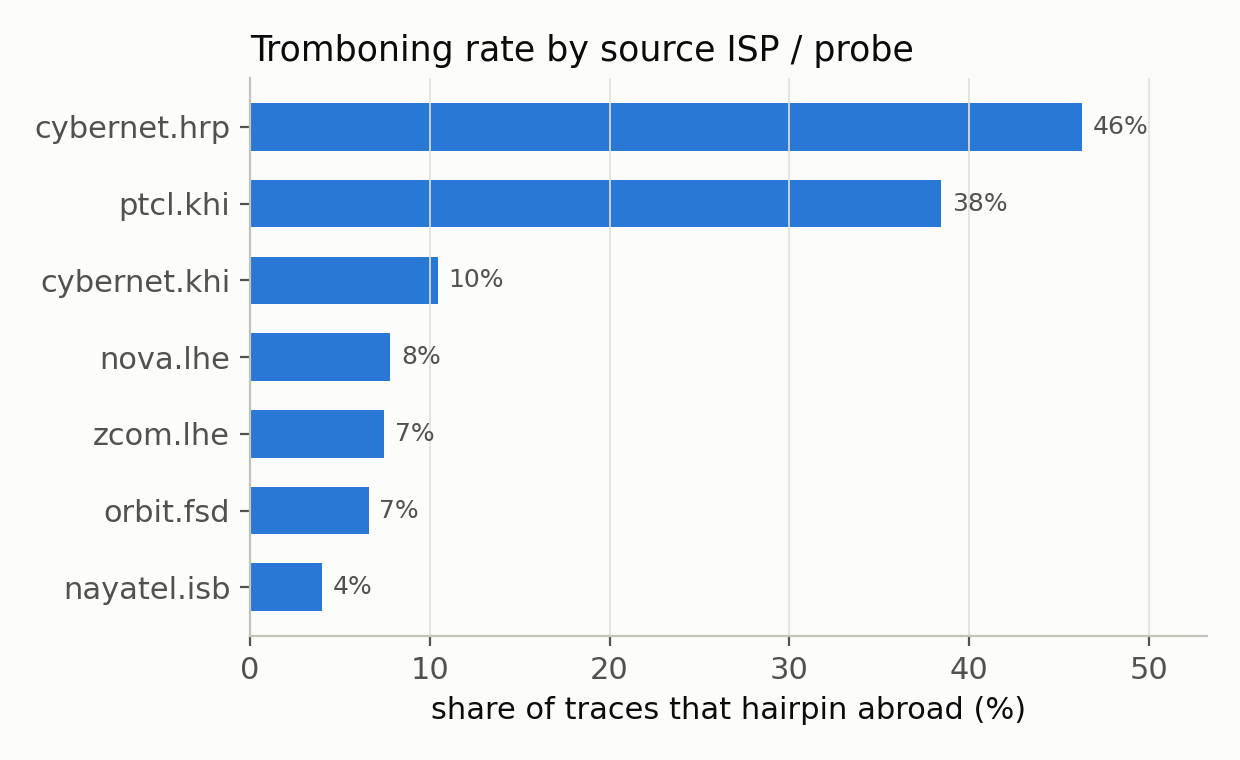
\includegraphics[width=\columnwidth]{fig_trombone_by_source.png}
  \caption{Tromboning rate by source ISP/probe. The outcome is dominated by \emph{where you
  measure from}, not the destination.}
  \label{fig:source}
\end{figure}

\begin{figure}[t]
  \centering
  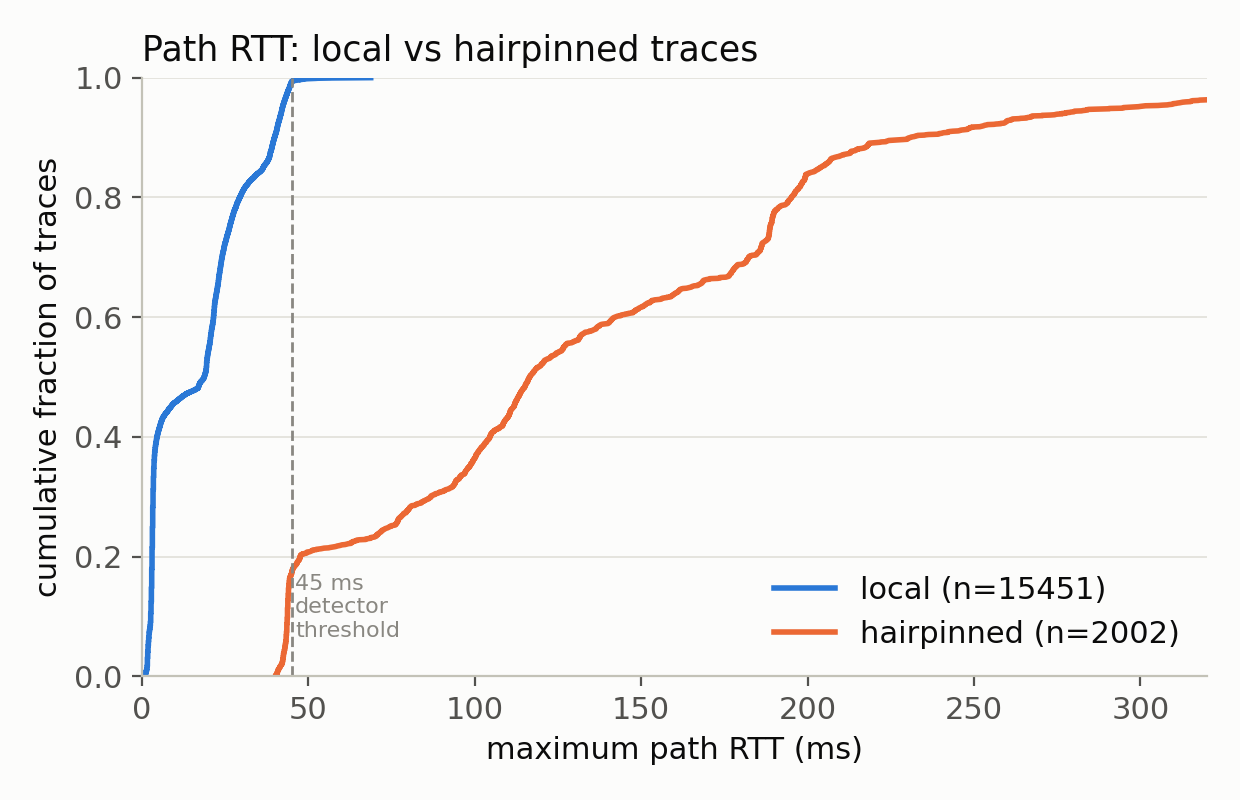
\includegraphics[width=\columnwidth]{fig_rtt_cdf.png}
  \caption{Distribution of maximum path RTT, local vs hairpinned traces. Local paths stay under
  the $45$\,ms detector threshold; hairpinned paths reach $100$--$300$\,ms. (The split at
  $45$\,ms is partly definitional; the informative content is the \emph{shape} of the hairpin
  curve.)}
  \label{fig:cdf}
\end{figure}

\begin{figure*}[t]
  \centering
  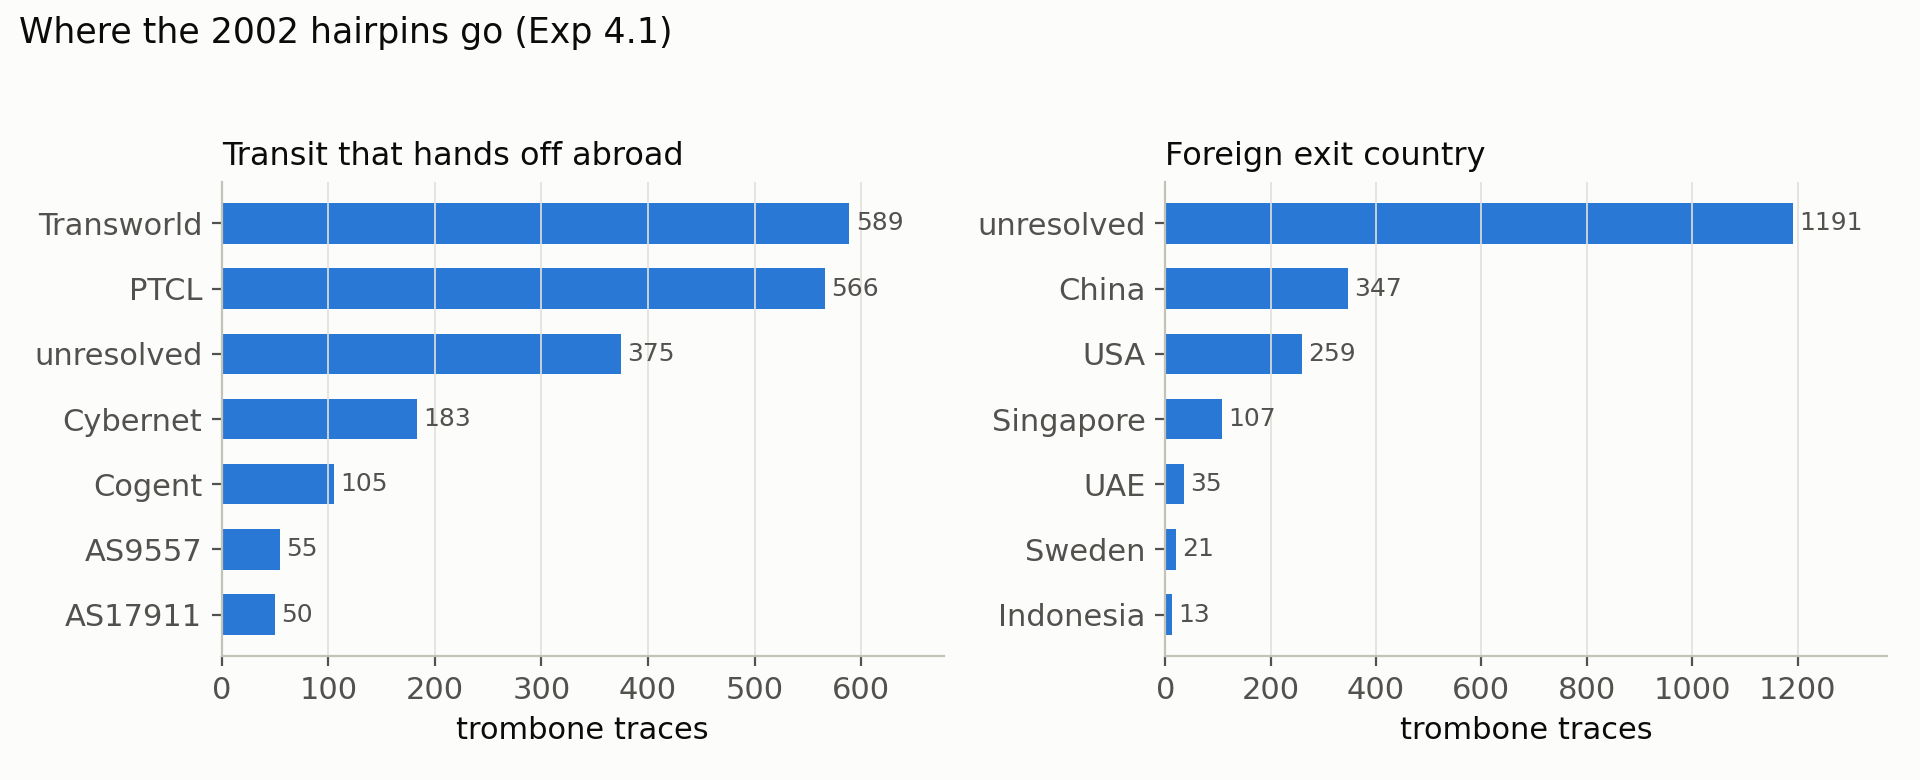
\includegraphics[width=\textwidth]{fig_trombone_transit_exit.png}
  \caption{Where the $2{,}002$ hairpins go: the transit that hands off abroad (Transworld
  ${\approx}$ PTCL) and the foreign exit country. ``Unresolved'' are RTT-proven trombones whose
  foreign hop did not answer.}
  \label{fig:transit}
\end{figure*}

\section{The Latency Cost and the Unused Local Path}
\label{sec:penalty}
\emph{Provenance: this is the longitudinal \textbf{pilot} (legacy ICMP Paris + ping, RTT
re-derived as min-of-$N$); the uniform, per-ISP four-indicator version is deferred to the
longitudinal panel (Sec.~\ref{sec:conclusion}).}

The hairpin has a price, and it is stable. Re-tracing a fixed panel every 15~minutes over days,
local Pakistani sites sit at $2$--$40$\,ms while two banks sit at $127$\,ms (MCB, served from
Singapore) and $200$\,ms (HBL, New Jersey)---a $3$--$9\times$ penalty that holds on every ISP.
The penalty shows \textbf{no diurnal cycle} and the routes are essentially static, so it is
\textbf{structural}---a hosting and peering choice, not evening congestion---and the fix is
local hosting and better peering, not more bandwidth. Routing quality is also unequal
\emph{within} the country: the same local site is $1.6$\,ms on Z-Com but $42$\,ms on Cybernet.

Why does the hairpin happen even between domestic parties? Because the transit structure forces
it: downstream ISPs route ${\sim}100\%$ of paths through an international operator (Z-Com
$91/91$, Nova $65/65$), whereas \textbf{Nayatel is only ${\sim}40\%$}---the most independent,
reaching CDNs and peers directly and using an operator only for genuinely foreign destinations.
A direct probe-to-probe test isolates the mechanism: \textbf{PTCL peers with Transworld
domestically in $100\%$ of local measurements but never ($0\%$) for abroad-hosted traffic}---the
peering exists, but only for local exchange. The domestic path is there; it is simply not the
one chosen for most flows.

\section{The Resilience Cost: a Submarine-Cable Fault}
\label{sec:cut}
On 2~July~2026 a fault on the \textbf{SMW5} submarine cable degraded Pakistan's international
capacity; traffic was rerouted onto surviving cables. We monitored ping + traceroute every
15~minutes for 12~hours from all 14 probes to a balanced CDN/Abroad/PK sample. It was a
\textbf{latency degradation, not a blackout}, and it \textbf{eased over the window}---worst-hit
paths collapsed from the outage peak (e.g.\ \texttt{shophive.com} via PTCL $646 \to 278$\,ms),
improving even as measurement moved into peak business hours, so the recovery is genuine and not
diurnal.

Quantified---outage peak (first 3\,h) vs recovered state (last 3\,h), international
targets---the fault hit as \textbf{instability, not a uniform latency step}
(Table~\ref{tab:impact}), concentrated on \textbf{PTCL-sourced paths} (RTT $+12\%$, jitter
$+50\%$). Path changes were \textbf{load-balancing within the same transit} (e.g.\ alternating
between two Etisalat-UAE ingress IPs), \emph{not} a reroute onto a different cable---the exit
country stayed constant, consistent with congestion on the SMW5-era detour easing rather than a
repair. Crucially, \textbf{local/PK-hosted targets showed no increase}---the disruption was
confined to the international leg. The single practical lesson: a cable cut badly hurts the
offshore-hosted majority and barely touches anything hosted in Pakistan and exchanged locally.

\begin{table}[t]
  \centering
  \caption{SMW5 outage impact, international targets: outage peak (first 3\,h) vs recovered
  (last 3\,h). No pre-event baseline, so the true rise vs a normal day is likely larger.
  Robust to the RTT definition: on min-of-$N$ RTT the change is $+0\%$ / jitter $+24\%$ ---
  same conclusion. Hop counts exclude ICMP-filtered / container probes.}
  \label{tab:impact}
  \begin{tabular}{lcc}
    \toprule
    Metric & Outage $\to$ recovered & Change \\
    \midrule
    Mean RTT      & $148 \to 145$\,ms   & $+2\%$ \\
    Jitter        & $13.6 \to 10.3$\,ms & $\mathbf{+31\%}$ \\
    Path length   & $28.6 \to 30.0$ hops & ${\sim}$flat \\
    Packet loss   & $10\% \to 11\%$     & ${\sim}$flat \\
    \bottomrule
  \end{tabular}
\end{table}

\section{Discussion}
The four results compose one argument. Content is largely offshore
(\S\ref{sec:host}); even domestic traffic hairpins abroad, by choice, through the two
international operators (\S\ref{sec:tromb}); this costs a stable $3$--$9\times$ latency penalty
and forgoes an available local path (\S\ref{sec:penalty}); and it removes a resilience margin
that local exchange would keep during a cable fault (\S\ref{sec:cut}). PKIX is the instrument
that closes all four---its own latency table ($1$--$31$\,ms vs $100$--$144$\,ms) shows the
gain---and the obstacle is not construction but \emph{use}: physical presence at PKIX is not
route exchange. In a three-set framing (Set~1 absent, Set~2 present but not peering, Set~3
actively exchanging), Wateen is a measured Set-2 example---listed at all three PKIX sites yet
routing to Cloudflare's Hong Kong PoP at $25$\,ms while Nayatel reaches it at $3$\,ms. Our
tromboning map is, in effect, a map of Set-1/2 behaviour at national scale. We do not yet
quantify forex saved: RIPE Atlas cannot see byte volume, so we report latency and resilience,
and leave a traffic-weighted cost estimate to future work.

\section{Conclusion and Future Work}
\label{sec:conclusion}
Measured from inside Pakistan, the country's Internet exchange is underused in a way that is
visible on the wire and costly to users: ${\sim}40\%$ of top content is offshore, $11\%$ of
small-ISP space is reachable only by hairpinning abroad, the hairpin is a routing choice with a
stable $3$--$9\times$ latency penalty, and it forfeits resilience during a cable fault. The
local path exists but is not taken. \textbf{Next:} repeat the census over days to range-bound
the $11\%$ and separate per-host from time-flipping routing; and run a \textbf{20-day,
all-probe longitudinal panel} over CDN/Abroad/PK sites and known tromboning IPs, under the
single mature framework, to deliver the \textbf{uniform four-indicator (RTT, hop count, jitter,
loss) per-ISP comparison} that our earlier snapshots cannot support, plus diurnal and weekly
stability and a normal-day baseline that captures the next cable fault with a true
before/during/after.

\section*{Acknowledgment}
Supported by the APNIC Foundation and supervised by Dr.\ Saqib Ilyas at LUMS. Measurements use
the RIPE Atlas platform.

\begin{thebibliography}{99}
\bibitem{dibartolomeo2015} M.~Di Bartolomeo, G.~Di Battista, R.~di Lallo, and C.~Squarcella,
``Is it really worth to peer at IXPs? A comparative study,'' in \emph{Proc. IEEE ISCC}, 2015.
\bibitem{gupta2014} A.~Gupta, M.~Calder, N.~Feamster, M.~Chetty, E.~Calandro, and
E.~Katz-Bassett, ``Peering at the Internet's frontier: A first look at ISP interconnectivity in
Africa,'' in \emph{Proc. PAM}, 2014.
\bibitem{klick2016} J.~Klick, S.~Lau, M.~W\"ahlisch, and V.~Roth, ``Selective, prefix-based
scanning of the IPv4 address space,'' in \emph{Proc. ACM IMC}, 2016. % verify exact title
\bibitem{ager2012} B.~Ager, N.~Chatzis, A.~Feldmann, N.~Sarrar, S.~Uhlig, and W.~Willinger,
``Anatomy of a large European IXP,'' in \emph{Proc. ACM SIGCOMM}, 2012.
\bibitem{chatzis2013} N.~Chatzis, G.~Smaragdakis, A.~Feldmann, and W.~Willinger, ``There is more
to IXPs than meets the eye,'' \emph{ACM SIGCOMM Comput. Commun. Rev.}, 2013.
\bibitem{sanchez2014} M.~A.~Sanchez et al., ``Inter-domain traffic estimation for the
outsider,'' in \emph{Proc. ACM IMC}, 2014.
\bibitem{ripeatlas} RIPE NCC, ``RIPE Atlas,'' \url{https://atlas.ripe.net/}.
\bibitem{ripestat} RIPE NCC, ``RIPEstat,'' \url{https://stat.ripe.net/}.
\bibitem{pta2026} Pakistan Telecommunication Authority, ``Pakistan Peering Roadshow,''
presentation, 2026.
\end{thebibliography}

\end{document}
